\chapter{理论研究}

此处格式已按模板设定,作者只需选择段落区域,输入替换之。模版中所有说明性文字用于注释格式与内容的要求,撰写论文时请删除。模版中,图表、公式、参考文献等都已给出范例,撰写论文时请删除。

本模版已包含符合章节设置的“多级别列表”,只需在相应位置替换标题文字即可。如需增加章节,建议先使用格式刷,再调整编号。

\section{毕业设计(论文)结构及要求}

\subsection{论文结构}

毕业设计(论文)原则上应采用中文完成(教学语言为英语的除外),确需用其他语言撰写的需经学院审批同意并报教务处备案。毕业设计(论文)一般由以下部分组成,依次为:①封面;②扉页;③独创性声明;④中英文摘要及关键词;⑤目录;⑥正文;⑦参考文献;⑧附录;⑨致谢。

\subsection{语言表述}

要做到数据可靠、推理严谨、立论正确。论述必须简明扼要、重点突出,对同行专业人员已熟知的常识性内容,尽量减少叙述。

论文中如出现一些非通用性的新名词、术语或概念,需做出解释。

\subsection{标题和层次}

标题要重点突出,简明扼要,层次要清楚。

\subsection{打印规格}

论文一律采用A4纸张(大小为210mm×297mm)打印,可根据实际选择单面或双面印刷,页边距如下设置。上:27.5mm;下:25.4mm;左:35.7mm;右:27.7mm。页眉距边界15.0mm;页脚距边界17.5mm。字符间距为默认值(缩放100\%,间距:标准)。


\section{毕业设计(论文)撰写规范}

\subsection{封面}

采用天津大学本科生毕业设计(论文)统一封面,封面内容包括论文题目、学院、专业、年级、姓名、学号、指导教师等信息。

论文题目是论文总体内容的体现,要求醒目、简明、准确,主题突出,一般不宜超过25字。

\subsection{目录}

目录的各章节应简明扼要,应列至三级标题,包含正文及其后的各部分,并附有相应页码。目录的文字应与相应标题文字完全一致。

“目录”两字之间空一个全角空格或两个半角空格,采用不编号章标题样式。目录条目采用正文样式。

各级标题采用逐级缩进形式,每级缩进2字符,页码前导符采用“…”。

\subsection{正文}

正文是毕业设计(论文)的主体,应占据主要篇幅,文字一般不少于15000字,要求主题明确,内容充实;论点正确,论据可靠,论证充分。内容一般包括:设计(论文)的工作目的(背景),国内外研究现状、理论分析、计算方法、实验装置和测试方法、实验结果分析与讨论、研究成果、结论及意义等。

正文中文字体为宋体,英文字体为Times New Roman,正文采用小四号字,段落行间距为固定值20磅,段落前后间距为0,首行缩进2字符。西文字体以Times New Roman为准,若Times New Roman中没有相应字符,则应使用较为清晰和通用的字体。数学公式和专门文字(如计算机程序代码)的字体可以根据需要选择。

章节与标号:一般分为章标题(一级标题)、不编号章标题(同属于一级标题)、二级标题和三级标题。各章节编号建议采用Word的“多级别列表”方式自动形成编号,标题编号与标题内容之间空一个全角空格或两个半角空格。各级章节标题格式要求细节参见《天津大学本科生毕业设计(论文)撰写规范》。

图、表等与其前后的正文之间要有一行的间距;文中的图、表、公式一律采用阿拉伯数字分章编号,如:图2-5,表3-2,公式(5-1)(“公式”两个字不要写上)等。若图或表中有附注,采用英文小写字母顺序编号。子图采用英文字母编号。引用图或表应在图题或表题右上角标出文献来源。图或表的附注应位于图或表的下方。

\subsection{公式}

公式要标准、通用,公式的变量和参数,除了公知公认的以外,一般要给出解释。文中的公式一律采用阿拉伯数字分章编号,如:公式(5-1)(“公式”两个字不要写上)。公式编号只能用于行间公式。公式编号右对齐,且应加英文小括号,不加引导符。其余样式与正文相同。变量和参数,不能采用正文格式,必须正确使用数学格式或行内公式格式,包含行内公式的段落可以采用单倍行距。

依照以上标准的行间公式范例如下。
%
\begin{equation}
  \left\{
    \begin{aligned}
      F_{si} &= k_{si}(z_i' - z_i) + c_{si}(\dot{z}_i' - \dot{z}_i) \\
      F_{ti} &= k_{ti}(z_i-y_i(x_i, t)) + c_{ti}(\dot{z}_i'-\dot{y}_i(x_i, t))
    \end{aligned}
  \right.
  \label{eq:F}
\end{equation}

其中:zi为车辆第i个轮胎由静平衡位置起算的竖向位移;yi为桥梁在第i个轮胎作用下的瞬时变位。

\subsection{图}

图要精选、简明,切忌与表及文字表述重复。图中的术语、符号、单位等应同文字表述一致。图与其前后的正文之间要有一行的间距;文中的图一律采用阿拉伯数字分章编号,如:图2-5。若图中有附注,采用英文小写字母顺序编号。子图采用英文字母编号。图序及图题居中置于图的下方,图、表内容为五号字,中文字体为宋体,英文字体为Times New Roman。图序与图题之间空一个全角空格或两个半角空格。引用图应在图题右上角标出文献来源。图的附注应位于图或表的下方。

依照以上标准的插图范例如下。


\begin{figure}[!htbp]
  \centering
  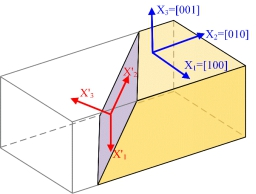
\includegraphics[width=0.6\textwidth]{figures/sample1.png}
  \caption{晶体坐标系和样品坐标系示意图}
  \label{fig:sample1}
\end{figure}

\begin{figure}[!htbp]
  \centering
  \subfloat[云图;]{
    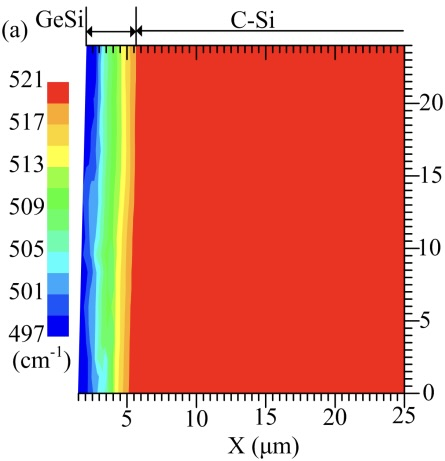
\includegraphics[height=0.38\textwidth]{figures/sample2L.jpeg}
  }
  \subfloat[沿深度方向分布曲线]{
    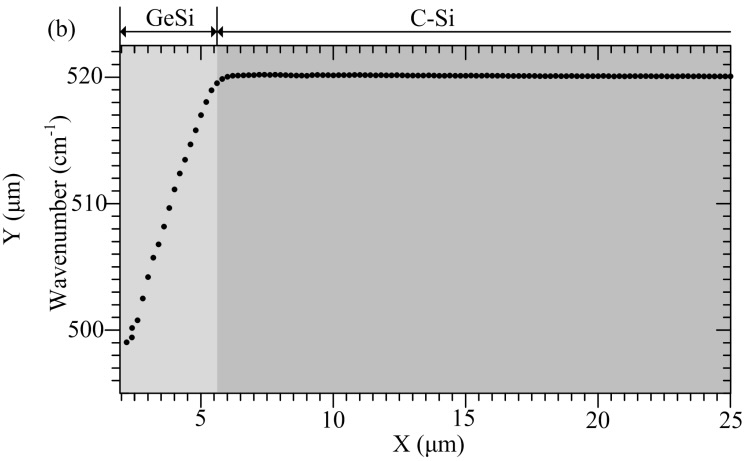
\includegraphics[height=0.38\textwidth]{figures/sample2R.jpeg}
  }
  \caption{应变硅横截面样品的拉曼类硅峰峰位}
  \label{fig:sample2}
\end{figure}


\subsection{表}

表中参数应标明量和单位的符号。表的编排建议采用国际通行的三线表。表与其前后的正文之间要有一行的间距;文中的表一律采用阿拉伯数字分章编号,如:表3-2。若表中有附注,采用英文小写字母顺序编号。表序及表题居中置于表的上方。如某个表需要转页接排,在随后的各页上应重复表序,后跟表题(可省略)和“(续)”,置于表格上方。续表均应重复表头。表序与表题之间空一个全角空格或两个半角空格。引用表应在表题右上角标出文献来源。表的附注应位于图或表的下方。

依照以上标准的三线表范例如下。

\begin{table}[!htbp]
  \centering
  \caption{典型微尺度力学实验方法的基本信息}
  \label{tab:tab1}
  \vspace{0.5em}
  \begin{tabular}{ccc}
    \toprule
    \textbf{实验方法} & \textbf{主要测量对象} & \textbf{空间分辨率}    \\
    \midrule
    原子力显微镜        & 表面力             & 0.1 nm {[}1{]}    \\
    透射电镜          & 晶格结构、位错         & 0.1 nm {[}2{]}    \\
    X射线衍射         & 应变              & 1 $\mu$m{[}3-5{]}     \\
    同步辐射          & 内部三维结构与变形       & 约100 nm{[}6, 7{]} \\
    显微拉曼          & 应变              & 250 nm {[}8{]}    \\ 
    \bottomrule
  \end{tabular}
\end{table}

\section{脚注}

在正文当中\footnote{脚注字号为五号,其余样式与正文相同。},如果有个别名词或情况需要解释时,可加注释说明。注释说明应采用文中编号加脚注的模式。脚注应采用阿拉伯数字上标,字体为Times New Roman,分页连续标号。脚注字号为五号,其余样式与正文相同。


\section{页眉和页脚}

页眉从正文开始到毕业设计(论文)结尾,一律设为“天津大学XX届本科生毕业设计(论文)”,采用五号字居中书写,其余样式与正文相同。

页脚从中文摘要开始,从 I 开始顺序编页码,为大写罗马数字格式。正文第一页开始,用阿拉伯数字重新从1开始顺序编页码,至学位论文结尾。页脚的字号为小五号,居中书写。
